\section{Experiments}
\label{sec:experiments}

We evaluate three questions.
(Q1)~Does the block-ordered mediator model recover the classifier-scale
effects when the true mediator law is known?
(Q2)~Does the parity constraint close more of the mediated disparity than
ordinary actionable recourse with the same cost, actions, validity level, and
intervention model?
(Q3)~When the method abstains, do the compatibility diagnostics of
Section~\ref{sec:theory} explain why?
(Q4)~How do these answers depend on the validity level $\gamma$ and on the
strength of the mediated effect?

% ---------------------------------------------------------------------------
\subsection{Experimental Design}
\label{sec:exp_design}

\paragraph{Datasets.}
We use one semi-synthetic benchmark with known mediator mechanisms and three
real datasets (Table~\ref{tab:datasets}).
\emph{German-Synth} adapts the semi-synthetic German Credit SCM
of~\citet{karimi2020imperfect} so that the true $P(W\mid X,Z)$ is available
and satisfies Assumptions~\ref{ass:ident} and~\ref{ass:intervene} by
construction.
\emph{Law School} (race), \emph{ACS Income} (sex), and \emph{Adult} (sex)
are standard fairness benchmarks whose mediators are, respectively, purely
continuous, mixed, and purely categorical. Data sources, preprocessing, the
full role assignment, and each mediator's actionability grid are in
Appendix~\ref{app:data}.

\begin{table}[t]
\centering
\small
\caption{Datasets. $|Z|$ counts pre-treatment covariates; mediator blocks are
listed in causal order, with $[\cdot]$ grouping an unordered block
(D: categorical, C: continuous). $n$ is the train/validation size of one
split.}
\label{tab:datasets}
\begin{tabular}{lllll}
\hline
Dataset & $X$ & $|Z|$ & Mediator blocks & $n$ (train / val) \\
\hline
German-Synth & sex  & 1 & D $\to$ D $\to$ D $\to$ [C,\,C] & 8{,}000 / 2{,}000 \\
Law School   & race & 2 & [C,\,C]                         & 14{,}955 / 3{,}739 \\
ACS Income   & sex  & 2 & D $\to$ D $\to$ [C,\,C]         & 241{,}218 / 60{,}305 \\
Adult        & sex  & 2 & D $\to$ D $\to$ D               & 36{,}177 / 9{,}045 \\
\hline
\end{tabular}
\end{table}

\paragraph{Classifiers.}
For each dataset we fit logistic regression ($C=1$), a multilayer perceptron
with hidden layers of 64 and 32 units and early stopping, and a random forest
(300 trees, minimum leaf size 20, $\sqrt{d}$ features per split), all with
scikit-learn~\citep{pedregosa2011scikit} on the training split. Categorical mediators are one-hot encoded and
continuous features standardized inside each classifier pipeline. The
decision threshold is $\tau=0.5$ throughout. Each classifier is held fixed
once trained; recourse acts on it and never retrains it.

\paragraph{Protocol and uncertainty.}
Every result is repeated over five seeds (42--46). Each seed redraws the
train/validation split and refits the mediator model and all classifiers
before recomputing every downstream quantity, so the spread across seeds
reflects the full pipeline. (German-Synth draws a single pool of 10{,}000
units from the SCM; seeds vary the split and all fits.) Recourse recipients
are the disadvantaged-group true negatives of the validation split
(Section~\ref{sec:intervention}). When there are more than 250 we draw 250
uniformly at random. Law School has only 33--46 per split and classifier, and
we use all of them. We report the mean $\pm$ standard deviation across the five seeds.
Within-seed percentile-bootstrap intervals, which hold the fitted models fixed,
are reported in Appendix~\ref{app:results}.

\paragraph{Mediator model implementation.}
The continuous block $f_\theta$ is a conditional autoregressive
rational-quadratic neural spline flow~\citep{durkan2019neural}, implemented
with the \texttt{nflows} library (v0.14;~\citealp{nflows}) on
PyTorch~\citep{paszke2019pytorch}. Each flow layer is a
\texttt{MaskedPiecewiseRationalQuadraticAutoregressiveTransform} with 8 bins,
linear tails outside $[-3,3]$, and a conditioner made of two residual
MADE blocks~\citep{germain2015made} of width 64. Successive layers are
separated by random permutations, and the base distribution is a standard
normal. Before fitting, each continuous mediator is mapped to a standard
normal marginal with a quantile transform fitted on the training split. All
samples are mapped back to natural units before they enter $\hat f$. Each
discrete head $g_\phi$ is a two-layer ReLU network (64 units) whose input is
$(x,\tilde z)$ concatenated with 4-dimensional embeddings of its parent
categories. Both factors are trained jointly on~\eqref{eq:flow_training} with
Adam (learning rate $10^{-3}$, halved after 5 epochs without validation
improvement), batch size 256, and gradient-norm clipping at 1.
Appendix~\ref{app:training} lists the per-dataset architecture.

\paragraph{Checkpoint selection.}
Validation likelihood alone is a poor guide here: every downstream quantity is
a Monte Carlo average over \emph{samples} from the model, and a checkpoint can
have good likelihood while producing biased mediator marginals, particularly for
small groups. After every epoch we therefore run a posterior-predictive check
on the validation split. For each validation context $(x_i,z_i)$ in a fixed
subset (4{,}096 contexts with 8 draws each on ACS and Adult; 2{,}000 with 16
on German-Synth) we draw mediator vectors from the model and compare them
with the observed mediators on five discrepancies:
(i)~the total-variation distance between the generated and observed marginal
of each categorical mediator, overall and
(ii)~within each group of $X$;
(iii)~for ordinal mediators, the $W_1$ distance between category codes
normalized by the number of categories minus one;
(iv)~the $W_1$ distance for each continuous mediator, normalized by its
observed standard deviation, overall and within each group; and
(v)~the largest absolute error in the pairwise correlations between continuous
mediators. A checkpoint is \emph{eligible} only if every discrepancy is below a
preset threshold. Among eligible checkpoints we keep the one minimizing
validation negative log-likelihood plus a weighted sum of the discrepancies.
Early stopping counts epochs without improvement only after the first eligible
checkpoint. A run in which no checkpoint is eligible is reported as a failure
and not used. Appendix~\ref{app:training} lists the thresholds for each
dataset. Law School selects on validation likelihood alone.
% TODO(author): state why Law School has no posterior-predictive gates, and
% whether the gate thresholds were fixed before the recourse experiments.

\paragraph{Monte Carlo estimation.}
All quantities are plug-in Monte Carlo estimates under the fitted mediator
model.
\emph{Effects.} We draw $n=500$ validation instances without replacement
and, for each, $K=500$ samples from $\hat P(W\mid X=b,z)$ for each mediator
arm $b\in\{0,1\}$. The same draws $w^{(k)}_b$ are evaluated under both
$a\in\{0,1\}$ in~\eqref{eq:mu_mc}. These common random numbers cancel the
mediator sampling noise in $\widehat\NDE$. We sample each arm directly, with no
importance weighting.
\emph{Reference.} For each recipient we draw $K_{\mathrm{ref}}=200$ samples
from $\hat P(W\mid x^{(1)},z_i)$ and score them with $\hat f_0$. This one
empirical $R_{z_i}$ gives $\hat\mu_{\mathrm{ref}}(z_i)$ and is
shared by every candidate plan of that recipient, so plans are compared
against the same reference draws.
\emph{Plans.} For each plan $a\in\mathcal A(w_{0,i})$, which we enumerate
exhaustively, we draw $K_{\mathrm{int}}=32$ samples from $Q_a$ by ancestral
sampling with clamping (Section~\ref{sec:intervention}). Validity is the
fraction of the 32 scores at or above $\tau$, so $\gamma=0.5$ requires at
least 16 of 32. $\mathbb E[P_a]$ is their mean, and $W_1(P_a,R_{z_i})$ is the
exact one-dimensional distance between the two empirical score distributions.
Both recourse methods select from the same candidate draws, so the only
difference between them is the selection rule.
% TODO(author): report the Monte Carlo noise floor of the empirical W1 at
% (K_int, K_ref) = (32, 200), e.g., W1 between two independent draws of R_z,
% to justify epsilon = 0.1 against the O(K^{-1/2}) upward bias noted in
% Section~\ref{sec:recourse_selection}.

\paragraph{Recourse settings.}
Both methods use the cost~\eqref{eq:cost}, the actionability grids of
Appendix~\ref{app:roles}, the intervention law $Q_a$, and the abstention
rule of Section~\ref{sec:recourse_selection}. Ordinary actionable recourse
minimizes cost subject to $\gamma$-validity. Our method also imposes
$W_1(P_a,R_{z_i})\le\varepsilon$. The baseline thus shares our causal model,
action space, and Monte Carlo draws, which makes it considerably stronger
than actionable recourse as usually implemented
(Section~\ref{sec:recourse_selection}). The main results use $\gamma=0.5$ and
$\varepsilon=0.1$ for every dataset. Unacted coordinates in the acted block
keep their factual values.

\paragraph{Sensitivity to $\gamma$.}
The validity level decides which regime of Theorem~\ref{thm:val-par} a
recipient falls in, since $\varepsilon_\gamma(z)$ grows with $\gamma$. We
therefore repeat the comparison for
$\gamma\in\{0.5,0.6,0.7,0.8,0.9\}$ on every dataset, classifier, and seed.
Each value of $\gamma$ re-selects plans from the same candidate draws and
reference draws, so differences across $\gamma$ come from the selection rule
alone and not from Monte Carlo noise. For each $\gamma$ we also compute
$\hat\varepsilon_\gamma(z_i)$ exactly from the empirical reference with the
closed form of Proposition~\ref{prop:compat}, and we split our method's
abstentions into causes~(a)--(c) of Section~\ref{sec:theory}.

% ---------------------------------------------------------------------------
\subsection{Measuring Success}
\label{sec:exp_metric}

The goal of our method is not that recipients cross the decision boundary.
Ordinary recourse already achieves that. The goal is that, after acting, each
recipient's expected score sits where it would sit under the advantaged
group's mediator law. We therefore measure success on the scale of the
post-recourse mediated disparity $D_{\mathrm{post},i}$~\eqref{eq:dpost}.

\paragraph{Primary metric: recipient-level closure.}
For the $n$ recipients of one dataset, classifier, and seed,
\begin{equation*}
  \mathrm{Closure}
  \;=\;1-\frac{\sum_{i=1}^n|D_{\mathrm{post},i}|}{\sum_{i=1}^n|D^{\mathrm{fact}}_{\mathrm{pre},i}|}
\end{equation*}
\eqref{eq:closure}, where
$D^{\mathrm{fact}}_{\mathrm{pre},i}=\hat\mu_{\mathrm{ref}}(z_i)-\hat f_0(w_{0,i},z_i)$
and
$D_{\mathrm{post},i}=\hat\mu_{\mathrm{ref}}(z_i)-\widehat{\mathbb E}[P_{a^*_i}]$
use the same reference draws. Four properties make this the right yardstick.
First, the denominator uses each recipient's \emph{factual} score, the
baseline that recourse actually changes~\eqref{eq:dpost_decomp}, rather than
the population $\NIE$, since recipients are selected on their factual scores.
Second, absolute values are taken per recipient, so an undershoot for one
recipient cannot cancel an overshoot for another.
Third, every recipient is counted. An abstaining recipient keeps
$D_{\mathrm{post},i}=D^{\mathrm{fact}}_{\mathrm{pre},i}$ and contributes no
closure, so abstaining cannot inflate the score.
Fourth, the scale has fixed reference points:
$\mathrm{Closure}=1$ means every recipient lands exactly on their reference,
$\mathrm{Closure}=0$ means the absolute disparity is unchanged in total (for
example, when every recipient abstains), and $\mathrm{Closure}<0$ means
recourse \emph{increased} the absolute mediated disparity, which happens when
recipients are pushed past their reference by more than they started below it.

\paragraph{Comparison with the baseline.}
Both methods are evaluated on the same recipients with the same draws, so we
also report the paired gain
$\frac1n\sum_i\bigl(|D^{\mathrm{base}}_{\mathrm{post},i}|-|D_{\mathrm{post},i}|\bigr)$,
the average reduction in absolute post-recourse disparity per recipient.
It is positive when the parity constraint brings recipients closer to their
reference than ordinary recourse does.

\paragraph{Secondary metrics.}
\emph{Overshoot rate}: the fraction of recipients whose post-recourse
disparity has the opposite sign to their factual one,
$D_{\mathrm{post},i}\,D^{\mathrm{fact}}_{\mathrm{pre},i}<0$. Because
recipients nearly always start below their reference, this is essentially
$\Pr[D_{\mathrm{post},i}<0]$. We report it together with the mean overshoot
size $\frac1n\sum_i\max\{0,-\operatorname{sign}(D^{\mathrm{fact}}_{\mathrm{pre},i})\,D_{\mathrm{post},i}\}$,
since landing on a distributional target produces many small overshoots that
are harmless.
\emph{Abstention rate}: the fraction of recipients for whom the program is
infeasible.
\emph{Cost}: the mean of $c(a^*_i)$ over \emph{all} recipients, with
abstentions contributing zero.
\emph{Compatibility diagnostics} (Section~\ref{sec:evaluation}): the share of
recipients whose reference is itself $\gamma$-valid, the medians of
$\hat\varepsilon_\gamma(z_i)$ and $\hat\varepsilon_{\mathcal A}(z_i,w_{0,i})$,
and the share of recipients in each abstention cause~(a)--(c).

% ---------------------------------------------------------------------------
\subsection{Results on the Semi-Synthetic Benchmark}
\label{sec:exp_synth}

\paragraph{Effect recovery (Q1).}
Table~\ref{tab:oracle} compares the effects estimated with the fitted mediator
model against oracle estimates that use the true SCM mediator law with the
same classifier, instances, and $K$. Across all three classifiers and five
seeds the estimated $\NIE$ is within $0.002$ of the oracle on average, and
within $0.006$ in the worst seed. The $\NDE$ error is at most $0.0012$.
The mean errors are smaller than the between-seed standard deviation of the
estimated $\NIE$, so the mediator model is not the limiting source of error
when the projection is correct.

\begin{table}[t]
\centering
\small
\caption{German-Synth: classifier-scale effects estimated with the fitted
mediator model versus the oracle that samples from the true SCM mediator law
(same classifier, instances, and $K$). Mean $\pm$ SD over five seeds; the
last column is the largest absolute $\NIE$ error over seeds.}
\label{tab:oracle}
\begin{tabular}{lccccc}
\hline
& \multicolumn{2}{c}{$\NDE$} & \multicolumn{2}{c}{$\NIE$} & \\
Classifier & Model & Error & Model & Error & Max $|$Error$|$ \\
\hline
Logistic & .037 $\pm$ .003 & +.0004 $\pm$ .0004 & .191 $\pm$ .004 & +.0016 $\pm$ .0021 & .0037 \\
MLP      & .041 $\pm$ .010 & +.0002 $\pm$ .0008 & .186 $\pm$ .016 & +.0011 $\pm$ .0027 & .0053 \\
RF       & .030 $\pm$ .002 & +.0004 $\pm$ .0002 & .182 $\pm$ .003 & +.0020 $\pm$ .0024 & .0055 \\
\hline
\end{tabular}
\end{table}

\paragraph{Recourse (Q2).}
German-Synth is in the compatible regime: every recipient's reference is
itself $0.5$-valid ($\varepsilon_\gamma=0$) and every recipient has a valid
plan. Here the parity constraint behaves as intended
(Table~\ref{tab:main_results}, top). Ordinary recourse stops once validity
is reached and closes 72--76\% of the factual disparity. Our method closes
91--92\% at about 14\% higher cost, abstains for at most 1.4\% of recipients,
and reduces each recipient's absolute disparity by 0.08--0.10 on average. The
paired gain is positive in every seed for every classifier. The overshoot rate
rises from 15--17\% to 49--59\%, as expected when the target is a
distribution rather than a threshold: recipients now land \emph{around} their
reference rather than below it. The mean overshoot size stays near
$0.02$, well inside $\varepsilon$.

\paragraph{Stress test: strength of the mediated effect (Q1, Q4).}
To see how the method behaves as the mediated disparity grows or vanishes,
we rerun the full pipeline on three further versions of German-Synth. Each
multiplies every sex$\to$mediator coefficient by a scale $\kappa$, which
changes the $\NIE$ but leaves the female mediator law, the outcome equation,
and hence the $\NDE$ ($0.042$ on $P(Y=1)$) unchanged
(Appendix~\ref{app:data_sources}, Table~\ref{tab:synth_versions}).
$\kappa=0$ is a null case with no mediated effect, and $\kappa=1$ is the
benchmark above. Table~\ref{tab:stress} reports the range over the three
classifiers.

\begin{table}[t]
\centering
\small
\caption{German-Synth mediation stress test at $\gamma=0.5$,
$\varepsilon=0.1$. Each cell is the range over the three classifiers of the
five-seed mean. $\NIE$ is the oracle classifier-scale effect; Err.\ is the
mean fitted-minus-oracle $\NIE$. Gain is the paired reduction in
$|D_{\mathrm{post}}|$ relative to ordinary recourse.}
\label{tab:stress}
\setlength{\tabcolsep}{3pt}
\begin{tabular}{rcccccc}
\hline
& & & \multicolumn{2}{c}{Closure (\%)} & & \\
$\kappa$ & $\NIE$ & Err. & Ord. & Ours & Abst.\ (\%) & Gain \\
\hline
0.0 & $-$.001       & +.007--.008      & 63--68 & 61--69 & 29--39 & $-$.004--.004 \\
0.5 & .092--.098    & +.004--.005      & 77--80 & 86--87 & 7--9   & .029--.045 \\
1.0 & .180--.189    & +.001--.002      & 72--76 & 91--92 & 1      & .076--.100 \\
2.0 & .303--.315    & $-$.004--$-$.003 & 62--63 & 93--94 & 0      & .193--.210 \\
\hline
\end{tabular}
\end{table}


\begin{figure*}[t]
\centering
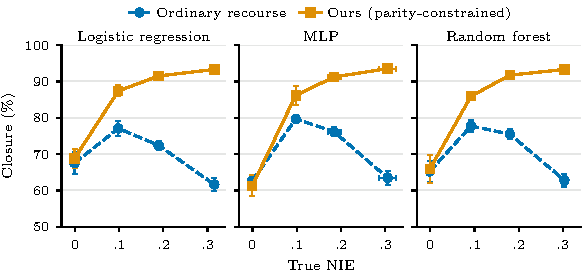
\includegraphics{figures/main/closure_vs_true_nie.pdf}\hfill
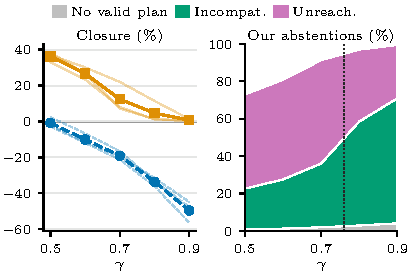
\includegraphics{figures/main/gamma_sensitivity.pdf}
\caption{(a)~German-Synth mediation stress test ($\gamma=0.5$,
$\varepsilon=0.1$), one panel per classifier. Each point is one version of
the benchmark, $\kappa\in\{0,0.5,1,2\}$ from left to right; the $\NDE$ is
$0.042$ in every version. The x-axis is the true $\NIE$ on the classifier
scale, computed by scoring the fitted classifier on mediators drawn from the
true SCM (500 validation instances, $K=500$ draws each). The y-axis is
recipient-level closure~\eqref{eq:closure} over the 250 disadvantaged-group
true negatives. Points are means over five seeds; error bars are $\pm1$ SD
across seeds in both coordinates. Dashed lines with circles show ordinary
recourse; solid lines with squares show our method.
(b)~ACS, sensitivity to the validity level $\gamma\in\{0.5,0.6,0.7,0.8,0.9\}$
($\varepsilon=0.1$). Both methods re-select plans from the same candidate and
reference draws at each $\gamma$. Left: recipient-level closure; thin lines
are the three classifiers (mean over five seeds) and thick lines their
average; the grey line marks zero closure. Right: our abstentions as a share
of all recipients, stacked by cause and averaged over classifiers and seeds:
no $\gamma$-valid plan (cause~(a) of Section~\ref{sec:theory}), target
incompatibility, $\varepsilon<\hat\varepsilon_\gamma(z)$ (cause~(b)), and
unreachability by the action grid (cause~(c)). The dotted line marks the
$\gamma$ at which the median $\hat\varepsilon_\gamma(z)$, averaged over
classifiers, reaches $\varepsilon$ (linear interpolation between grid
points, $\gamma\approx0.76$).}
\label{fig:main}
\end{figure*}

Figure~\ref{fig:main}(a) plots closure against the true $\NIE$.
Three patterns stand out. First, the gain over ordinary recourse grows with
the mediated effect, from zero in the null case to about $0.2$ per recipient
at $\kappa=2$. It is positive in every seed and for every classifier when
$\kappa>0$. Our closure rises with $\kappa$ (87\%, 92\%, 93\%), whereas
ordinary recourse's closure peaks at $\kappa=0.5$ and then falls. At small
$\kappa$ the reference sits close to the threshold, and ordinary recourse
overshoots it (69--78\% of recipients at $\kappa=0$). At large $\kappa$ the
reference sits far above the threshold, and ordinary recourse stops short of
it (overshoot 1--2\%). These are the two regimes of
Proposition~\ref{prop:overshoot}, and the parity constraint corrects
ordinary recourse in both directions.
Second, in the null case the method does no harm to closure, but it is not
free: it abstains for 29--39\% of recipients, all unreachable (cause~(c)).
With no mediated disparity, the reference is the disadvantaged group's own
mediator law at $z$, a wide score distribution that a single plan's narrower
distribution often cannot match within $\varepsilon$. Ordinary recourse
serves these recipients and lands on average no further from the reference.
Third, the mediator model is most biased, relative to the effect, when there
is no effect: it reports an $\NIE$ of about $0.008$ when the truth is zero. The
absolute error stays below $0.01$ at every $\kappa$, and the worst single
seed is $0.02$ at $\kappa=2$.

% ---------------------------------------------------------------------------
\subsection{Results on Real Data}
\label{sec:exp_real}

\begin{table*}[t]
\centering
\small
\caption{Recourse for disadvantaged-group true negatives at $\gamma=0.5$ and
$\varepsilon=0.1$. ``Ord.'' is ordinary actionable recourse; ``Ours'' adds the
distributional parity constraint. Closure is recipient-level
closure~\eqref{eq:closure} (higher is better; negative means recourse
increased the absolute mediated disparity). Gain is the paired reduction in
$|D_{\mathrm{post}}|$ relative to ordinary recourse. Ref.\ valid is the share
of recipients whose advantaged reference is $\gamma$-valid. Mean $\pm$ SD over
five complete refits; $n$ recipients per seed.}
\label{tab:main_results}
\setlength{\tabcolsep}{4pt}
\begin{tabular}{llr r cc cc cc c}
\hline
& & & &
\multicolumn{2}{c}{Closure (\%)} &
\multicolumn{2}{c}{Abstention (\%)} &
\multicolumn{2}{c}{Cost} & \\
Dataset & Clf. & $n$ & Ref.\ valid &
Ord. & Ours & Ord. & Ours & Ord. & Ours & Gain \\
\hline
German-Synth & LR  & 250 & 100\% & 72.4 $\pm$ 1.3 & \textbf{91.5} $\pm$ 0.8 & 0.0 & 1.4 & 0.66 & 0.75 & .100 $\pm$ .009 \\
             & MLP & 250 & 100\% & 76.1 $\pm$ 1.2 & \textbf{91.2} $\pm$ 0.4 & 0.0 & 1.4 & 0.65 & 0.74 & .076 $\pm$ .004 \\
             & RF  & 250 & 100\% & 75.5 $\pm$ 1.3 & \textbf{91.7} $\pm$ 0.5 & 0.0 & 1.0 & 0.65 & 0.75 & .081 $\pm$ .006 \\
\hline
Law School   & LR  & 40  & 100\% & 29.1 $\pm$ 1.5 & \textbf{87.4} $\pm$ 0.9 & 0.0 & 0.0 & 0.86 & 6.10 & .289 $\pm$ .007 \\
             & MLP & 43  & 100\% & 23.9 $\pm$ 5.3 & \textbf{78.8} $\pm$ 16.7 & 0.0 & 14.3 & 1.04 & 6.02 & .237 $\pm$ .071 \\
             & RF  & 38  & 100\% & 28.1 $\pm$ 3.6 & \textbf{85.1} $\pm$ 1.3 & 0.0 & 0.0 & 0.68 & 4.43 & .243 $\pm$ .016 \\
\hline
ACS Income   & LR  & 250 & 22\%  & $-$2.8 $\pm$ 6.5 & \textbf{37.0} $\pm$ 4.8 & 0.0 & 72.5 & 0.65 & 0.23 & .084 $\pm$ .018 \\
             & MLP & 250 & 22\%  & 2.3 $\pm$ 4.5    & \textbf{38.4} $\pm$ 5.0 & 0.9 & 72.4 & 1.11 & 0.27 & .078 $\pm$ .010 \\
             & RF  & 250 & 22\%  & $-$2.0 $\pm$ 10.7 & \textbf{33.0} $\pm$ 9.0 & 1.3 & 74.0 & 1.00 & 0.27 & .072 $\pm$ .018 \\
\hline
Adult        & LR  & 250 & 0\%   & $-$199.8 $\pm$ 28.9 & \textbf{0.0} $\pm$ 0.0 & 30.5 & 100.0 & 0.65 & 0.00 & .167 $\pm$ .020 \\
             & MLP & 250 & 0\%   & $-$247.6 $\pm$ 23.7 & \textbf{0.0} $\pm$ 0.0 & 35.7 & 100.0 & 0.53 & 0.00 & .180 $\pm$ .022 \\
             & RF  & 250 & 0\%   & $-$183.5 $\pm$ 3.0  & \textbf{0.0} $\pm$ 0.0 & 40.6 & 100.0 & 0.42 & 0.00 & .140 $\pm$ .008 \\
\hline
\end{tabular}
\end{table*}

The real datasets span the regimes that Theorem~\ref{thm:val-par}
separates, and the reference-validity column of Table~\ref{tab:main_results}
predicts where each one falls.

\paragraph{Compatible regime: Law School (Q2).}
On Law School the mediated disparity is large (pure $\NIE$ of $0.19$--$0.21$
against an $\NDE$ of $0.12$--$0.14$), and every recipient's reference is
$0.5$-valid. Ordinary recourse reaches validity and stops, closing only
24--29\% of the factual disparity and never overshooting. The parity
constraint raises closure to 79--87\%, and the paired gain is positive in
every seed. This is the regime in which, by
Proposition~\ref{prop:overshoot}, validity alone leaves disparity unclosed.
The price is cost: recipients are asked for roughly six to seven times more
change in LSAT and GPA (in standardized units), because reaching the
reference requires moving further than the boundary. The MLP's larger spread
comes from one seed in which 20 of its 41 recipients abstained. With so few
recipients, a single seed moves the mean noticeably. All of Law School's
abstentions are cause~(c): a valid plan exists and the reference is
compatible, but the action grid cannot reach within $\varepsilon$ of it.

\paragraph{Mixed regime: ACS (Q2, Q3).}
On ACS only 22\% of recipients have a $0.5$-valid reference, and the
compatibility threshold is small but positive for the rest (median
$\hat\varepsilon_\gamma=0.02$). Ordinary recourse overshoots the reference
for 81--84\% of recipients and, on balance, leaves the absolute disparity
where it started (closure between $-3$\% and $+2$\%). Our method serves the
26--28\% of
recipients for whom the target is attainable and abstains for the rest. Those
it serves land close enough to their reference to lift closure to 33--38\%,
and overshoot falls from 81--84\% to 16--17\%. Its average cost is lower
because abstaining recipients incur none.
The abstentions split into cause~(b), $\varepsilon<\hat\varepsilon_\gamma$
(20--23\% of recipients), and cause~(c), unreachable by the action grid
(48--52\%). Almost every recipient has some valid plan (cause~(a) is at
most 1.3\%).

\paragraph{Incompatible regime: Adult (Q3).}
On Adult \emph{no} recipient's reference is $0.5$-valid: on average only
3--4\% of the advantaged reference's scores clear $\tau$. By
Theorem~\ref{thm:val-par}, every valid plan must then sit at least
$\varepsilon_\gamma(z)>0$ from the reference, and ordinary recourse, which
must be valid, overshoots it for 44--53\% of recipients. On average this
overshoot is larger than the disparity they started with, so ordinary
recourse yields strongly \emph{negative} closure ($-184$\% to $-248$\%). Adult's
factual disparities are small (pure $\NIE\approx0.03$), which magnifies the
ratio. Our method abstains for every recipient: 31--41\% have no valid plan
(cause~(a)), 24--38\% face $\varepsilon<\hat\varepsilon_\gamma$ (cause~(b)),
and the remaining 32--35\% are unreachable (cause~(c)). Its closure is
therefore zero, and its paired gain comes entirely from \emph{not} pushing
recipients past their reference. We read this as a correct refusal, not as
successful recourse. Most of Adult's disparity runs through the direct path
($\NDE\approx0.13$ against a pure $\NIE$ of $0.02$--$0.03$), which
mediator-based recourse cannot reach.

% ---------------------------------------------------------------------------
\subsection{Sensitivity to the Validity Level}
\label{sec:exp_gamma}

We ran the $\gamma$ sweep on every dataset (Appendix~\ref{app:results}) and
report ACS in the main text because it is the only dataset that moves through
all three regimes as $\gamma$ grows (Table~\ref{tab:gamma_acs}). Raising
$\gamma$ moves the threshold up through the advantaged reference's score
distribution. The share of recipients with a $\gamma$-valid reference falls
from 22\% to zero by $\gamma=0.8$, and the median compatibility threshold
$\hat\varepsilon_\gamma$ rises from $0.02$ to $0.15$--$0.17$, past
$\varepsilon=0.1$ at $\gamma\approx0.8$.

\begin{table}[t]
\centering
\small
\caption{ACS, sensitivity to the validity level $\gamma$ ($\varepsilon=0.1$).
Ref.\ valid: share of recipients whose reference is $\gamma$-valid.
$\hat\varepsilon_\gamma$: median compatibility threshold. Abstention causes
for our method: (b)~$\varepsilon<\hat\varepsilon_\gamma$, (c)~unreachable;
cause~(a) is at most 7\% throughout. Percentages; mean over five seeds (SD
at most 12.7 points).}
\label{tab:gamma_acs}
\setlength{\tabcolsep}{3.5pt}
\begin{tabular}{llrrrrrrr}
\hline
& & & & \multicolumn{2}{c}{Closure} & & \multicolumn{2}{c}{Abst.\ cause} \\
Clf. & $\gamma$ & Ref.\ valid & $\hat\varepsilon_\gamma$ & Ord. & Ours & Abst. & (b) & (c) \\
\hline
LR  & 0.5 & 22.4 & .017 & $-$2.8  & 37.0 & 72.5 & 20.4 & 52.1 \\
    & 0.6 & 10.7 & .042 & $-$12.0 & 30.1 & 78.3 & 26.1 & 52.2 \\
    & 0.7 &  1.4 & .073 & $-$21.2 & 22.0 & 84.6 & 37.1 & 47.4 \\
    & 0.8 &  0.0 & .109 & $-$36.0 & 11.4 & 92.6 & 54.6 & 38.0 \\
    & 0.9 &  0.0 & .149 & $-$56.3 &  1.3 & 99.0 & 70.2 & 28.7 \\
\hline
MLP & 0.5 & 21.6 & .022 &    2.3  & 38.4 & 72.4 & 23.4 & 48.2 \\
    & 0.6 &  3.0 & .051 &  $-$6.6 & 26.6 & 81.7 & 27.3 & 52.8 \\
    & 0.7 &  0.1 & .087 & $-$16.6 &  7.1 & 95.2 & 36.6 & 55.8 \\
    & 0.8 &  0.0 & .128 & $-$33.2 &  1.3 & 99.1 & 59.9 & 34.9 \\
    & 0.9 &  0.0 & .173 & $-$47.7 &  0.6 & 99.6 & 67.0 & 26.9 \\
\hline
RF  & 0.5 & 21.6 & .018 &  $-$2.0 & 33.0 & 74.0 & 22.0 & 50.7 \\
    & 0.6 &  2.5 & .041 & $-$11.6 & 23.4 & 82.5 & 25.4 & 54.9 \\
    & 0.7 &  0.0 & .072 & $-$19.5 &  8.1 & 94.2 & 28.5 & 62.6 \\
    & 0.8 &  0.0 & .108 & $-$31.4 &  1.1 & 99.1 & 52.2 & 42.6 \\
    & 0.9 &  0.0 & .150 & $-$44.8 &  0.2 & 99.8 & 63.2 & 30.0 \\
\hline
\end{tabular}
\end{table}


Figure~\ref{fig:main}(b) summarizes the sweep.

\paragraph{The two methods fail in opposite directions (Q4).}
As $\gamma$ grows, ordinary recourse must push recipients further above
$\tau$, and its closure falls steadily, from about $0$ to between $-45$\%
(RF) and $-56$\% (LR). Each step up in $\gamma$ turns more of its recommendations into
over-corrections. Our method responds to the same change by abstaining more,
from 72--74\% to over 99\%, so its closure falls towards zero but never below it. The
paired gain over ordinary recourse stays positive at every $\gamma$
(0.05--0.12), because one method degrades by over-correcting while the other
degrades by declining to act.

\paragraph{The theory predicts the abstention mix (Q3, Q4).}
As $\gamma$ grows, abstentions shift from cause~(c) to cause~(b). At
$\gamma=0.5$ most abstentions are unreachability, a property of the action
grid. By $\gamma=0.9$, 63--70\% of recipients face a target that no valid
score distribution can meet, whatever the actions or the cost. The
crossing point matches the median $\hat\varepsilon_\gamma$ passing
$\varepsilon$. In every dataset, classifier, seed, and $\gamma$, the smallest
attainable $W_1$ among valid plans was at least $\hat\varepsilon_\gamma$, so the
lower bound of Theorem~\ref{thm:val-par} held in all 525 evaluations,
including the stress-test versions of German-Synth.

\paragraph{The other datasets.}
Law School is unaffected by $\gamma$. Its two mediators form a single block,
so a plan either clamps a mediator or keeps its factual value, $Q_a$ is a
point mass, and validity is 0 or 1 for every plan. Adult abstains for every
recipient at every $\gamma$, while ordinary recourse's closure worsens from
$-200$\% to $-234$\% (LR). German-Synth shows the limit of the method when
the reference is compatible but hard to reach. As $\gamma$ rises from 0.5 to
0.9 its references stop being valid (100\% to 9--12\%). Abstentions, all
cause~(c), grow from 1\% to 32--50\%. Our closure drops from 91--92\% to
52--65\%, below ordinary recourse's 77--78\%, and the paired gain turns
negative from $\gamma=0.8$ (MLP) or $0.9$ (LR, RF). When most recipients are
reachable only within a loose tolerance, a fixed $\varepsilon=0.1$ rejects
plans that ordinary recourse would accept and that would have closed most of
the gap. This argues for setting $\varepsilon$ jointly with $\gamma$, for
example as $\hat\varepsilon_\gamma(z)$ plus a margin, which we leave to future
work.

\paragraph{A tuned baseline.}
The sweep also lets us give ordinary recourse an advantage that our method
does not get. For each dataset and classifier we pick the $\gamma$ at which
ordinary recourse achieves its highest closure, choosing it after the fact on
the same recipients we evaluate on, and compare it with our method at the
fixed $\gamma=0.5$. This is an upper bound on what tuning $\gamma$ could do
for the baseline. Among the main datasets, tuning helps ordinary recourse only
on German-Synth, where
its best closure rises from 72--76\% to 81--82\%; it is still 10--11 points
below ours (91--92\%). On the stress-test versions with a mediated effect, the
tuned baseline trails our fixed-$\gamma$ method by 6.5--9 points at
$\kappa=0.5$ and 11--13 points at $\kappa=2$. On ACS, Adult, and Law School,
$\gamma=0.5$ is already the baseline's best level, so the margins in
Table~\ref{tab:main_results} stand. Only in the null case ($\kappa=0$) are
the two methods level (within 1.4 points either way), as they should be when
there is no mediated disparity to close.

\paragraph{Summary.}
When validity and parity are compatible, the parity constraint closes
substantially more of the mediated disparity than ordinary recourse, at a
higher cost and with small, bounded overshoot. When they are incompatible,
the theory predicts it, the diagnostics detect it, and the method abstains
instead of recommending actions that would over-correct. Ordinary recourse
has no such check: in that regime it widens the absolute mediated disparity it
was meant to address, and more so the stricter the validity requirement. The
main cost of our method is that a fixed tolerance $\varepsilon$ can be too
strict when $\gamma$ is high, as on German-Synth.
